% !TeX program = lualatex
\documentclass[fleqn]{NotesClass}

\strictpagecheck

\usepackage{csquotes}
\usepackage{subcaption}

\usepackage{tikz}
\usetikzlibrary{external}
\tikzexternalize[prefix=tikz-external/]

\usepackage{tikz-cd}
\AtBeginEnvironment{tikzcd}{\tikzexternaldisable}
\AtEndEnvironment{tikzcd}{\tikzexternalenable}

\usepackage[pdfauthor={Willoughby Seago},pdftitle={Notes from Algebraic Geometry Course},pdfkeywords={algebraic geometry},pdfsubject={Algebraic Geometry}]{hyperref}  % Should be loaded second last (cleveref last)
\colorlet{hyperrefcolor}{blue!60!black}
\hypersetup{colorlinks=true, linkcolor=hyperrefcolor, urlcolor=hyperrefcolor}
\usepackage[
capitalize,
nameinlink,
noabbrev
]{cleveref} % Should be loaded last

% My packages
\usepackage{NotesBoxes}
\usepackage{NotesMaths2}

\setmathfont[range={\int, \oint, \otimes, \oplus, \bigotimes, \bigoplus}]{Latin Modern Math}


% Highlight colour
\definecolor{my blue}{HTML}{084887}
\definecolor{my red}{HTML}{CA1551}
\definecolor{my green}{HTML}{17C3B2}
\definecolor{my yellow}{HTML}{F58A07}
\definecolor{my purple}{HTML}{CB9CF2}
\colorlet{highlight}{my green}

% Title page info
\title{Algebraic Geometry}
\author{Willoughby Seago}
\date{October 6th, 2025}
\subtitle{Notes from}
\subsubtitle{University of Glasgow}
\renewcommand{\abstracttext}{These are my notes from the SMSTC course \emph{Algebraic Geometry} taught by Dr Giulia Gugiatti and Prof Ivan Cheltsov. These notes were last updated at \printtime{} on \today{}.}

% Commands
% Maths
\newcommand{\subideal}{\triangleq}

\includeonly{}

\begin{document}
    \frontmatter
    \titlepage
    \innertitlepage{}
    \tableofcontents
    % \listoffigures
    \mainmatter
    
    \chapter{Introduction}
    
    \section{Conventions and Notation}
    Throughout the notes the ground field, \(K\), will always be assumed to be \emph{algebraically closed}, up to the point where we introduce schemes.
    Taking \(K = \complex\) is usually reasonable.
    
    All rings, \(R\), are assumed to be \emph{commutative} with \emph{unity}.
    That \(J\) is an ideal of \(R\) will be denoted \(J \subideal R\).
    The ideal generated by a subset, \(S \subseteq R\), is denoted \(\langle S \rangle\).
    
    \section{Motivation}
    This section contains various motivating examples of algebro-geometric thinking, in varying levels of precision.
    Since the goal is to motivate some precision may be lacking.
    
    \subsection{Systems of Polynomial Equations}
    When we first learned algebra in high school it was to study the zeros of polynomials.
    Later we learned linear algebra, which it can be argued is the study of the zeros of systems of linear equations.
    Algebraic geometry combines these two fundamental fields into the study of zeros of systems of polynomials.
    
    Given \(f_1, \dotsc, f_m \in K[x_1, \dotsc, x_n]\) the basic object of study of algebraic geometry is the \defineindex{affine variety}
    \begin{equation}
        X = \{x \in K^n \mid f_i(x) = 0 \text{ for } i = 1, \dotsc, m\}.
    \end{equation}
    What questions can we ask about this set?
    Just as a single complex polynomial, \(f \in \complex[x]\), cannot be solved exactly for \(\deg f > 4\) we cannot possibly hope to explicitly list the points in \(X\).
    Instead we reason about the geometric structure of the solutions.
    We will ask geometric questions about \(X\), which we then aim to answer by an algebraic study of the \(f_i\).
    
    In the following sections we will give several examples of the sorts of geometric objects which can arise.
    We will focus on the existence of connections to other areas of mathematics.
    
    \subsection{Riemann Surfaces}
    Fix some positive integer, \(n\).
    We can define a curve\footnote{Note that this is a \enquote{curve} since it's complex dimension is \(1\) (we'll define dimension of affine varieties later, for now just use your intuition for the dimension of a manifold). Of course, in our pictures this single complex dimension is drawn as two real dimensions.}
    \begin{equation}
        c_n = \{(x, y) \in \complex^2 \mid y^2 = (x - 1)(x - 2)(x - 3) \dotsm (x - 2n)\} \subseteq \complex^2.
    \end{equation}
    We can view the defining equation as defining the quantity \(y\).
    Since we have \(y^2 = \dotso\) to find the value of \(y\) we have to take a square root.
    What we get depends on the value of \(x\).
    For most cases, specifically \(x \ne 1, 2, \dotsc, 2n\), we have
    \begin{equation}
        y = \pm \sqrt{(x - 1)(x - 2) \dotsm (x - 2n)}.
    \end{equation}
    For \(x = 1, 2, \dotsc, 2n\) we have
    \begin{equation}
        y = 0.
    \end{equation}
    Consider what values \(y\) can take.
    For \(x \ne 1, \dotsc, 2n\) we have two copies of \(\complex\), one for \(+ \sqrt{(x-1) \dotsm (x - 2n)}\) and one for \(-\sqrt{(x - 1) \dotsm (x - 2n)}\).
    For \(x = 1, \dotsc, 2n\) we only have one possible value, \(0\).
    The picture this suggests is two copies of \(\complex\) identified at the points \(1, \dotsc, 2n\).
    
    However, this isn't quite right.
    We know that \(z \in \complex^{\times}\) doesn't have a distinguished choice of \(\sqrt{z}\).
    Upon passing once around the origin they are exchanged.
    For example, if we take the path \(x = r\e^{i\theta}\), with \(r \ge 0\) fixed and \(\theta \in [0, 2\pi]\) then \(\sqrt{x} = \sqrt{r} \e^{i\theta/2}\).
    Then at \(\theta = 0\) we get \(\sqrt{r}\) and at \(\theta = 2\pi\) we get \(-\sqrt{r}\).
    The result is that as we go around the points \(x = 1, \dotsc, 2n\) we move from one copy of \(\complex\) to the other.
    
    Fortunately, we know how to deal with this, we take branch cuts between zeros.
    Take both copies of \(\complex\), and perform branch cuts along the intervals \([1, 2], [3, 4], \dotsc, [2n - 1, 2n]\).
    For \(n = 3\) this produces \cref{fig:complex planes with branch cuts}.
    Now glue these along the cuts, which gives the picture
    % TODO
    Finally, because it makes things nicer, add two points at infinity, one for each copy of \(\complex\), compactifying everything to get the picture
    % TODO
    We see that this leaves us with a Riemann surface of genus \(g = n - 1\).
    
    \begin{figure}
        \centering
        \begin{subfigure}{0.8\textwidth}
            \tikzexternaldisable
            \tikzsetnextfilename{riemann-surface-1}
            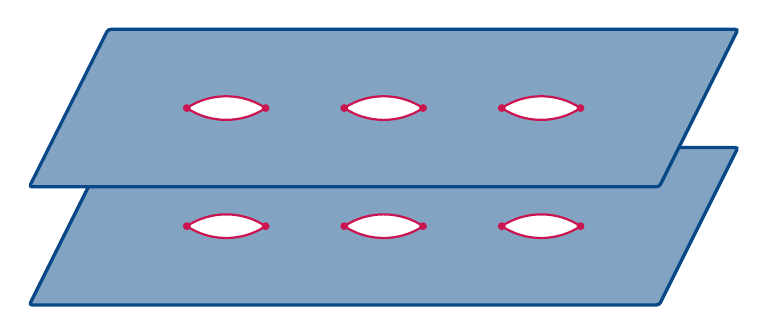
\begin{tikzpicture}
                \draw [very thick, rounded corners=1, my blue, fill=my blue!50] (0, -2) -- (8, -2) -- (9, 0) -- (1, 0) -- cycle;
                \draw [very thick, rounded corners=1, my blue, fill=my blue!50] (0, -0.5) -- (8, -0.5) -- (9, 1.5) -- (1, 1.5) -- cycle;
                
                \foreach \i in {1, 3, 5} {
                    \fill [white]  (1 + \i, 0.5) .. controls (1.3 + \i, 0.7) and (1.7 + \i, 0.7) .. (2 + \i, 0.5) .. controls (1.7 + \i, 0.3) and (1.3 + \i, 0.3) .. (1 + \i, 0.5);
                    \fill [white] (1 + \i, -1) .. controls (1.3 + \i, -0.8) and (1.7 + \i, -0.8) .. (2 + \i, -1) .. controls (1.7 + \i, -1.2) and (1.3 + \i, -1.2) .. (1 + \i, -1);
                    \draw [thick, my red] (1 + \i, 0.5) .. controls (1.3 + \i, 0.7) and (1.7 + \i, 0.7) .. (2 + \i, 0.5);
                    \draw [thick, my red] (1 + \i, 0.5) .. controls (1.3 + \i, 0.3) and (1.7 + \i, 0.3) .. (2 + \i, 0.5);
                    \draw [thick, my red] (1 + \i, -1) .. controls (1.3 + \i, -0.8) and (1.7 + \i, -0.8) .. (2 + \i, -1);
                    \draw [thick, my red] (1 + \i, -1) .. controls (1.3 + \i, -1.2) and (1.7 + \i, -1.2) .. (2 + \i, -1);
                }
                \foreach \i in {1, 2, 3, 4, 5, 6} {
                    \fill [my red] (1 + \i, 0.5) circle [radius=0.05];
                    \fill [my red] (1 + \i, -1) circle [radius=0.05];
                }
            \end{tikzpicture}
            \caption{Branch cuts along alternate intervals.}
            \label{fig:complex planes with branch cuts}
        \end{subfigure}
        \caption{Producing a Riemann surface from a curve}
    \end{figure}
    
    \backmatter
    \renewcommand{\glossaryname}{Acronyms}
    \printglossary[acronym]
    \printindex
\end{document}